\documentclass[11pt]{article}

% ----- preamble -----
\usepackage[a4paper,margin=1.8cm]{geometry}
\usepackage{amsmath,amssymb}
\usepackage{alltt}
\usepackage{tikz}
\usepackage{tikz-cd}
\usetikzlibrary{arrows.meta,positioning,calc,fit,backgrounds,
  shapes.geometric,chains,decorations.pathreplacing}
\usepackage[most]{tcolorbox}
\usepackage{parskip}
\usepackage{xcolor}

\definecolor{ink}{RGB}{40,40,40}
\definecolor{soft}{RGB}{245,245,248}
\definecolor{kas}{RGB}{30,110,190}
\definecolor{grn}{RGB}{30,140,80}

% the three brick colours
\definecolor{faceL}{RGB}{30,140,80}   % linearized trace loop  L
\definecolor{faceF}{RGB}{200,140,0}   % Frobenius / doubling   F
\definecolor{faceC}{RGB}{130,70,170}  % cyclotomic coset       C
\definecolor{comb}{RGB}{30,110,190}   % combinators
\definecolor{asm}{RGB}{190,50,60}     % assembly / results

\newtcolorbox{note}[1][]{colback=soft,colframe=ink,boxrule=0.4pt,
  arc=2pt,left=6pt,right=6pt,top=4pt,bottom=4pt,#1}
\newtcolorbox{leanbox}[1][]{colback=black!4,colframe=black!55,boxrule=0.4pt,
  arc=1.5pt,left=5pt,right=5pt,top=3pt,bottom=3pt,#1}

% code block: alltt keeps ^ _ % $ literal, but \( \) { } still give math/groups
\newenvironment{lean}{\begin{leanbox}\begin{alltt}\small}{\end{alltt}\end{leanbox}}

\tikzset{
  obj/.style={draw=ink,rounded corners=3pt,fill=soft,inner sep=5pt,font=\small,align=center},
  brick/.style={draw=ink,rounded corners=2pt,inner sep=6pt,font=\small,align=center,
    minimum height=13mm},
  thm/.style={draw=ink,rounded corners=3pt,fill=white,inner sep=4pt,
    font=\small,align=center,minimum height=9mm},
  arr/.style={-{Stealth[length=2.5mm]},thick},
  dep/.style={-{Stealth[length=2.4mm]},thick,ink},
  badge/.style={circle,inner sep=0pt,minimum size=3.8mm,font=\scriptsize\bfseries,text=white},
}
\newcommand{\bL}{\tikz[baseline=-0.6ex]\node[badge,fill=faceL]{L};}
\newcommand{\bF}{\tikz[baseline=-0.6ex]\node[badge,fill=faceF]{F};}
\newcommand{\bC}{\tikz[baseline=-0.6ex]\node[badge,fill=faceC]{C};}
\newcommand{\ck}{\textcolor{grn}{\checkmark}}
\newcommand{\lc}[1]{\texttt{\small #1}}

\title{\vspace{-1.5cm}\textbf{How the \texttt{Kasami} modules are built from the LEGO blocks}\\[4pt]
\large Bricks \bL\ \bF\ \bC\ $\to$ combinators $\to$ the Kasami map $\to$ the permutation criterion}
\author{\small A picture book of the \texttt{Kasami} Lean library (Lean\,/\,Mathlib) --- \texttt{import Kasami}}
\date{}

\begin{document}
\maketitle
\vspace{-1.0cm}

\begin{note}
\textbf{What this note is.} The \texttt{Kasami/} library is a block-structured
re-presentation of the \emph{permutation half} of Dobbertin's 1999 paper
\emph{Kasami Power Functions, Permutation Polynomials and Cyclic Difference Sets}.
The design is deliberately LEGO-like: fix three primitive \textbf{bricks} (the maps
\bL\ \bF\ \bC), add a few \textbf{combinators} that snap them together, then
\textbf{assemble} the Kasami map and read off the headline permutation criterion by
pure composition. Every box drawn below is a \ck\ \emph{sorry}-free Lean
declaration (standard axioms \lc{propext}, \lc{Classical.choice}, \lc{Quot.sound}
only). This document describes the current \texttt{Kasami/} modules, not the older
\texttt{Equation1/} extract (which is the reused engine underneath).
\end{note}

%=====================================================================
\section*{The architecture at a glance}

\begin{center}
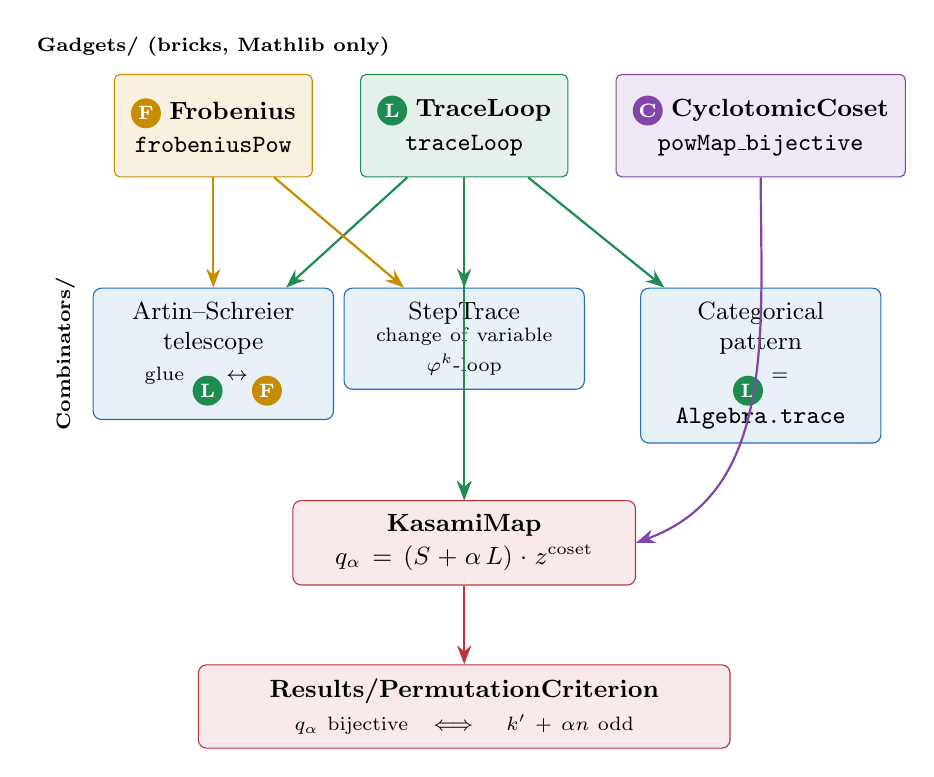
\begin{tikzpicture}[node distance=6mm]
% bricks layer
\node[brick,draw=faceL,fill=faceL!12] (L) {\bL\ \textbf{TraceLoop}\\[1pt]\scriptsize\lc{traceLoop}};
\node[brick,draw=faceF,fill=faceF!12,left=of L] (F) {\bF\ \textbf{Frobenius}\\[1pt]\scriptsize\lc{frobeniusPow}};
\node[brick,draw=faceC,fill=faceC!12,right=of L] (C) {\bC\ \textbf{CyclotomicCoset}\\[1pt]\scriptsize\lc{powMap\_bijective}};
\node[above=1mm of F,font=\scriptsize\bfseries] {Gadgets/ (bricks, Mathlib only)};

% combinators layer
\node[obj,draw=comb,fill=comb!10,below=14mm of F,text width=27mm] (AS)
  {Artin--Schreier\\ telescope\\ \scriptsize glue \bL\,$\leftrightarrow$\,\bF};
\node[obj,draw=comb,fill=comb!10,below=14mm of L,text width=27mm] (ST)
  {StepTrace\\ \scriptsize change of variable\\ \scriptsize $\varphi^k$-loop};
\node[obj,draw=comb,fill=comb!10,below=14mm of C,text width=27mm] (CT)
  {Categorical\\ pattern\\ \scriptsize \bL\ $=$ \lc{Algebra.trace}};
\node[left=1mm of AS,font=\scriptsize\bfseries,rotate=90,anchor=south] {Combinators/};

% assembly
\node[obj,draw=asm,fill=asm!10,below=14mm of ST,text width=40mm] (KM)
  {\textbf{KasamiMap}\\[1pt] $q_\alpha=(S+\alpha\,L)\cdot z^{\text{coset}}$};
\node[obj,draw=asm,fill=asm!10,below=10mm of KM,text width=64mm] (RES)
  {\textbf{Results/PermutationCriterion}\\[1pt]
  \scriptsize$q_\alpha$ bijective $\iff k'+\alpha n$ odd};

% edges bricks -> combinators
\draw[dep,faceF] (F) -- (AS);  \draw[dep,faceL] (L) -- (AS);
\draw[dep,faceF] (F) -- (ST);  \draw[dep,faceL] (L) -- (ST);
\draw[dep,faceL] (L) -- (CT);
% combinators + bricks -> KasamiMap
\draw[dep] (ST) -- (KM);
\draw[dep,faceL] (L.south) to[out=-90,in=90] (KM.north);
\draw[dep,faceC] (C.south) to[out=-90,in=20] (KM.east);
% KasamiMap -> results
\draw[dep,asm] (KM) -- (RES);
\end{tikzpicture}
\end{center}

\noindent The dependency edges are literal Lean \lc{import}s. The \bC\ brick and
\bL\ brick feed the assembly directly (the coset power and the $\alpha L$ term);
the \bF/\bL\ combinators supply the numerator engine $S$ and the telescoping
identities that the underlying root-counting argument consumes.

%=====================================================================
\section{The three bricks --- \texttt{Kasami/Gadgets/}}

Each brick depends on \emph{Mathlib only}, so all three are reusable and
upstreamable on their own.

\subsection*{\bF\ Frobenius / doubling --- \texttt{Gadgets/Frobenius.lean}}
The inserted map $\varphi:x\mapsto x^{2}$ and its iterates $\varphi^r:x\mapsto x^{2^r}$
(``doubling on the exponent''). Closing law and cycling are the arithmetic that
brick \bC\ later turns into orbit combinatorics.
\begin{lean}
def frobenius (x : F) : F := x ^ p          -- \(\varphi\): x \(\mapsto\) x^p  (p=2: doubling)
def frobeniusPow (r : \(\mathbb{N}\)) (x : F) : F := x ^ (p ^ r)   -- \(\varphi\)^r
frob_cycle           : x ^ Fintype.card F = x          -- closing law (Fermat) \ck
frobeniusPow_periodic: |F|=p^n \(\Rightarrow\) \(\varphi\)^r x = \(\varphi\)^(r % n) x   \ck
frobeniusPow_bijective: Function.Bijective (frobeniusPow p r)  \ck
\end{lean}

\subsection*{\bL\ Linearized trace loop --- \texttt{Gadgets/TraceLoop.lean}}
The Frobenius map \emph{closed into a loop}: $L_m(x)=\sum_{i<m}x^{2^i}$. Additive,
Frobenius-equivariant, and at full length idempotent (a bit).
\begin{center}
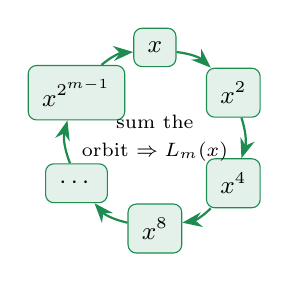
\begin{tikzpicture}[scale=1,every node/.style={font=\small}]
\def\R{1.15}
\foreach \a/\lab in {90/x,30/x^2,-30/x^4,-90/x^8,-150/\cdots,150/x^{2^{m-1}}}{
  \node[obj,draw=faceL,fill=faceL!12] (n\a) at (\a:\R) {$\lab$};}
\draw[arr,faceL] (n90) to[bend left=18] (n30);
\draw[arr,faceL] (n30) to[bend left=18] (n-30);
\draw[arr,faceL] (n-30) to[bend left=18] (n-90);
\draw[arr,faceL] (n-90) to[bend left=18] (n-150);
\draw[arr,faceL] (n-150) to[bend left=18] (n150);
\draw[arr,faceL] (n150) to[bend left=18] (n90);
\node[align=center] at (0,0) {\scriptsize sum the\\[-1pt]\scriptsize orbit $\Rightarrow L_m(x)$};
\end{tikzpicture}
\end{center}
\begin{lean}
def traceLoop (m : \(\mathbb{N}\)) (x : F) : F := \(\sum\)\_{i<m} x ^ (2 ^ i)
traceLoop_add      : traceLoop m (x+y) = traceLoop m x + traceLoop m y   \ck  -- additive
traceLoop_frobenius: traceLoop m (x^2) = (traceLoop m x)^2               \ck  -- equivariant
traceLoop_sq       : |F|=2^n \(\Rightarrow\) (traceLoop n x)^2 = traceLoop n x       \ck  -- idempotent
traceLoop_isBit    : |F|=2^n \(\Rightarrow\) traceLoop n x = 0 \(\vee\) traceLoop n x = 1   \ck  -- a bit
\end{lean}

\subsection*{\bC\ Cyclotomic-coset bookkeeping --- \texttt{Gadgets/CyclotomicCoset.lean}}
Where \bF\ cycles a \emph{point}, \bC\ cycles an \emph{exponent}: $\times 2$ permutes
$\mathbb{Z}/(2^n-1)$, its orbits are the cyclotomic cosets. Two arithmetic facts and one
permutation criterion are consumed downstream.
\begin{lean}
mersenne_coprime : Coprime k n \(\Rightarrow\) Coprime (2^k-1) (2^n-1)          \ck
inv_mod_exists   : Coprime k n \(\Rightarrow\) 1<2^n-1 \(\Rightarrow\) \(\exists\)b,(2^k-1)*b % (2^n-1)=1  \ck
powMap_bijective : Coprime (|F|-1) a \(\Rightarrow\) 0<a \(\Rightarrow\)
                     Function.Bijective (fun x => x ^ a)               \ck
\end{lean}

%=====================================================================
\section{The combinators --- \texttt{Kasami/Combinators/}}

A combinator snaps bricks together. Three of them.

\subsection*{Artin--Schreier telescope --- glue \bL\ to \bF}
Inserting the doubling map into the loop makes it telescope: the loop turns the
Artin--Schreier element $x^2+x$ into a single Frobenius difference.
\begin{center}
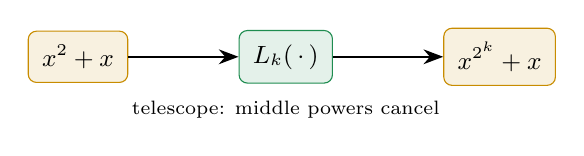
\begin{tikzpicture}[node distance=7mm,every node/.style={font=\small}]
\node[obj,draw=faceF,fill=faceF!12] (x) {$x^2+x$};
\node[obj,draw=faceL,fill=faceL!12,right=14mm of x] (L) {$L_k(\,\cdot\,)$};
\node[obj,draw=faceF,fill=faceF!12,right=14mm of L] (out) {$x^{2^k}+x$};
\draw[arr] (x)--(L); \draw[arr] (L)--(out);
\node[below=1mm of L,font=\scriptsize] {telescope: middle powers cancel};
\end{tikzpicture}
\end{center}
\begin{lean}
traceLoop_artin_schreier         : traceLoop k (x^2+x) = x^(2^k)+x        \ck
traceLoop_frobenius_invariant    : |F|=2^n \(\Rightarrow\) traceLoop n (x^(2^k)) = traceLoop n x  \ck
traceLoop_artin_schreier_zero    : |F|=2^n \(\Rightarrow\) traceLoop n (t^(2^k)+t) = 0    \ck
\end{lean}

\subsection*{StepTrace --- linearized change of variable}
Insert $\varphi^k:x\mapsto x^{2^k}$ instead of $\varphi$ and close \emph{that} into a loop:
the step-$2^k$ partial trace $P_{k,k'}(x)=\sum_{j<k'}x^{2^{jk}}$. This is the
\textbf{numerator engine} of the Kasami map.
\begin{lean}
def stepTrace (k k' : \(\mathbb{N}\)) (x : F) : F := \(\sum\)\_{j<k'} x ^ (2 ^ (j*k))     -- P
def numeratorSum (k k' : \(\mathbb{N}\)) (x : F) : F := \(\sum\)\_{i=1..k'} x ^ (2^(i*k)) -- S
stepTrace_add                 : stepTrace k k' (x+y) = \(\ldots\)x + \(\ldots\)y   \ck  -- linearized
numeratorSum_eq_stepTrace_frob: numeratorSum k k' x = (stepTrace k k' x)^(2^k)  \ck
stepTrace_telescope           : (stepTrace k k' x)^(2^k)+stepTrace k k' x
                                  = x^(2^(k'*k))+x                          \ck
\end{lean}

\subsection*{Categorical trace pattern --- \bL\ \emph{is} the field trace}
The loop is not ad hoc: it is Mathlib's \lc{Algebra.trace}, the single
``open $\to$ insert $\to$ close $\to$ keep what returns'' move applied to the
field's multiplication maps.
\begin{center}
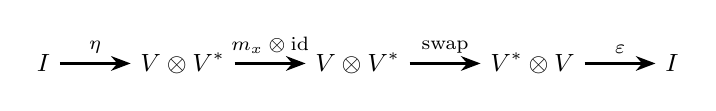
\begin{tikzpicture}[node distance=9mm,font=\small]
\node (I) {$I$};
\node[right=of I] (V) {$V\otimes V^*$};
\node[right=of V] (VV) {$V\otimes V^*$};
\node[right=of VV] (Vs) {$V^*\otimes V$};
\node[right=of Vs] (I2) {$I$};
\draw[arr] (I)--node[above,font=\scriptsize]{$\eta$}(V);
\draw[arr] (V)--node[above,font=\scriptsize]{$m_x\otimes\mathrm{id}$}(VV);
\draw[arr] (VV)--node[above,font=\scriptsize]{swap}(Vs);
\draw[arr] (Vs)--node[above,font=\scriptsize]{$\varepsilon$}(I2);
\end{tikzpicture}
\end{center}
\begin{lean}
traceLoop_eq_algebraMap_trace :
  traceLoop (finrank (ZMod 2) L) x
    = algebraMap (ZMod 2) L (Algebra.trace (ZMod 2) L x)              \ck
\end{lean}

%=====================================================================
\section{The assembly --- \texttt{Kasami/KasamiMap.lean}}

The generalized Kasami polynomial is the three bricks snapped together:
\[
q_\alpha(z)\;=\;\big(\underbrace{S_{k,k'}(z)}_{\text{\lc{numeratorSum} \bF/\bL}}
  \;+\;\alpha\cdot\underbrace{L_n(z)}_{\text{\lc{traceLoop} \bL}}\big)\;\cdot\;
  z^{\,(2^n-1)-(2^k+1)}_{\phantom{X}\text{\lc{coset power} \bC}} .
\]
\begin{center}
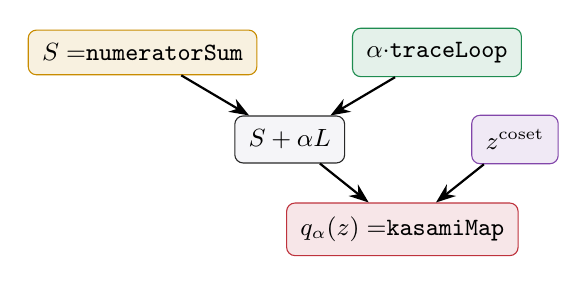
\begin{tikzpicture}[node distance=9mm,font=\small]
\node[obj,draw=faceF,fill=faceF!12] (S) {$S=$\lc{numeratorSum}};
\node[obj,draw=faceL,fill=faceL!12,right=12mm of S] (aL) {$\alpha\cdot$\lc{traceLoop}};
\node[obj,draw=ink,fill=soft,below=8mm of $(S)!0.5!(aL)$] (plus) {$S+\alpha L$};
\node[obj,draw=faceC,fill=faceC!12,right=16mm of plus] (pw) {$z^{\text{coset}}$};
\node[obj,draw=asm,fill=asm!12,below=8mm of $(plus)!0.5!(pw)$] (q) {$q_\alpha(z)=$\lc{kasamiMap}};
\draw[arr] (S)--(plus); \draw[arr] (aL)--(plus);
\draw[arr] (plus)--(q); \draw[arr] (pw)--(q);
\end{tikzpicture}
\end{center}
\begin{lean}
def kasamiMap (n k k' \(\alpha\) : \(\mathbb{N}\)) (z : F) : F :=
  (numeratorSum k k' z + (\(\alpha\):F) * traceLoop n z) * z ^ (2^n - 1 - (2^k + 1))
kasamiMap_zero_pt : kasamiMap n k k' \(\alpha\) 0 = 0      \ck  -- fixes 0
kasamiMap_eq_qKasami : kasamiMap n k k' \(\alpha\) z = qKasami n k k' \(\alpha\) z   \ck  -- rfl
\end{lean}
The map is \emph{definitionally} the paper's \lc{qKasami}, so the permutation
criterion proved for the underlying engine transfers verbatim.

%=====================================================================
\section{The result --- \texttt{Kasami/Results/PermutationCriterion.lean}}

The headline (Dobbertin's Theorem~1), read off by composition:

\begin{center}
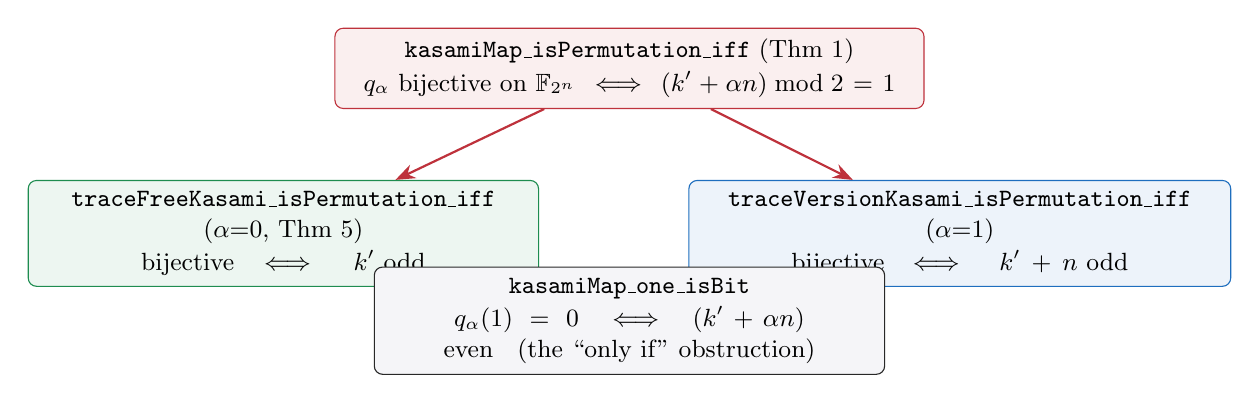
\begin{tikzpicture}[node distance=7mm,font=\small]
\node[thm,draw=asm,fill=asm!8,text width=72mm] (T1)
  {\textbf{\lc{kasamiMap\_isPermutation\_iff}} (Thm 1)\\[1pt]
   $q_\alpha$ bijective on $\mathbb{F}_{2^n}\iff (k'+\alpha n)\bmod 2 = 1$};
\node[thm,draw=faceL,fill=faceL!8,below left=9mm and -26mm of T1,text width=62mm] (T5)
  {\textbf{\lc{traceFreeKasami\_isPermutation\_iff}} ($\alpha{=}0$, Thm 5)\\[1pt]
   bijective $\iff k'$ odd};
\node[thm,draw=comb,fill=comb!8,below right=9mm and -30mm of T1,text width=66mm] (T1a)
  {\textbf{\lc{traceVersionKasami\_isPermutation\_iff}} ($\alpha{=}1$)\\[1pt]
   bijective $\iff k'+n$ odd};
\node[thm,draw=ink,fill=soft,below=20mm of T1,text width=62mm] (One)
  {\textbf{\lc{kasamiMap\_one\_isBit}}\\[1pt]
   $q_\alpha(1)=0\iff (k'+\alpha n)$ even \; (the ``only if'' obstruction)};
\draw[arr,asm] (T1)--(T5); \draw[arr,asm] (T1)--(T1a);
\end{tikzpicture}
\end{center}
\begin{lean}
theorem kasamiMap_isPermutation_iff (hn : |F|=2^n) (hk : k<n)
    (hcop : Coprime k n) (hk' : k*k' % n = 1 % n) (hk0 : 0<k)
    (hexp : 2^k+1 < 2^n-1) (\(\alpha\) : \(\mathbb{N}\)) (h\(\alpha\) : \(\alpha\)=0 \(\vee\) \(\alpha\)=1) :
  Function.Bijective (kasamiMap n k k' \(\alpha\)) \(\iff\) (k' + \(\alpha\)*n) % 2 = 1   \ck
\end{lean}

\begin{note}
\textbf{Verdict.} Yes --- the permutation half of Dobbertin's paper genuinely
factors through this compositional toolkit. The three bricks \bL\ \bF\ \bC\ plus
the three combinators (Artin--Schreier telescope, step-$2^k$ change of variable,
categorical pattern) assemble the Kasami map and deliver Theorem~1 and its two
cases. The heavy root-counting argument they compose over lives in the reused,
already \emph{sorry}-free \texttt{Equation1/} engine; this \texttt{Kasami/} layer
is its readable, block-structured re-presentation.

\textbf{Scope.} This covers the \emph{permutation} half only (Theorem~1, Theorem~5,
the trace-version case). The difference-set half (autocorrelation, 2-rank, the
\S3--4 conjecture) needs two further primitives not built here --- a
Fibonacci-style recursion block for the explicit inverse, and a character/Fourier
block $\psi=(-1)^{\mathrm{Tr}}$ --- whose hard content is not delivered by
composition alone.
\end{note}

\end{document}
